\section{\anglicismo{Redshift} fotométrico de ETGs a partir de \spire}\label{sec:3_redshift_hatlas}

En esta sección se describe un método válido para estimar el \rt\ fotométrico de las ETGs a partir de las medidas del instrumento \spire\ del satélite espacial \h.  El método se basa en el hecho de que las ETGs poseen el máximo absoluto de emisión en el IR-lejano, sobre los \microm{100} para el sistema en reposo, debido a la emisión IR por parte del gas y polvo interestelar; dado que las medidas del \spire\ se encuentran a \microm{250}, \microm{350} y \microm{500}, estas coinciden en torno al máximo cuando \maths{1\lesssim z\lesssim3.5}. 

Se considera que a la emisión IR de las galaxias \anglicismo{starburst} contribuyen tres componentes diferentes, dependiendo del entorno astrofísico en que se originó: nubes moleculares, nubes difusas de baja densidad (cirros) y regiones circunucleares calentadas por el Núcleo Galáctico Activo (AGN) \citep{article:Lapi_2011}. De las tres, la componente \comillas{caliente}, procedente de las nubes de gas moleculares, es la que resulta relevante para el ajuste que se va llevar a cabo, debido a que es la componente más intensa en la zona del espectro en la que \spire\ realiza las medidas. En el rango de \maths{\lambda \sim 50-500\;\mu \mathrm{m}} (considerando el sistema en reposo), la SED de las galaxias \anglicismo{starburst} típicas puede modelarse (mostrando diferencias de entorno al \maths{10\%-20\%}) como suma de dos cuerpos grises\footnote{Puede encontrarse mucha más información sobre la ecuaciones del cuerpo gris en el artículo \cite{article:cuerpo_gris}.}  siendo el flujo \maths{{S}_{\nu}}, para cada uno de ellos, 

\begin{equation}
{S}_{\nu} \propto \frac{{\nu}^{3+\beta}}{\exp{\frac{h\nu}{K{T}_{d}}}-1},
\end{equation}

con temperaturas \maths{{T}_{d}\approx30\;\mathrm{K}} y \maths{{T}_{d}\approx60\;\mathrm{K}} y unos índices de emisividad para el polvo de \maths{\beta=1.7} y \maths{\beta=2} respectivamente. 
A diferencia de la mayoría de los algoritmos para determinar el \rt\ fotométrico, el método propuesto tomará como única referencia la SED de la galaxia \smm. Como veremos, esta decisión se fundamenta en los estudios realizados por \cite{article:Nuevo_2012} y \cite{article:Lapi_2011}. 

\subsection{Selección de la SED de referencia}\label{sec:selecion_sed} 

La idea de obtener el \rt\ fotométrico a partir de la SED de la galaxia \smm\ no es nuestra y las razones para elegir la SED de esta galaxia en concreto se explican con detalle en \cite{article:Lapi_2011}. Estos autores seleccionaron un conjunto de cuatro galaxias que consideraron representativas de las galaxias en formación típicas y cuya SED se encuentra bien determinada e hicieron varios estudios para saber cual era la SED más adecuada para realizar los ajustes. Para ello, en primer lugar identificaron las posibles fuentes de error a la hora de realizar el ajuste y consideraron que había dos fuentes de error principales.

La primera fuente de error está relacionada con el hecho de que resolución angular de los instrumentos de medida es menor cuanto mayor es la longitud de onda. Por este motivo la radiación electromagnética procedente de una fuente, tiende a mezclarse con la procedente de las fuentes próximas, lo cuál produce un incremento del flujo medido respecto del valor real. Para cuantificar el efecto que producen las fuentes débiles sobre las medidas del flujo llevaron a cabo simulaciones \cite{article:Rigby_2011} que muestran \porcentaje{56.5} de las fuentes detectadas a \maths{\geqslant\!5\;\sigma} a \microm{500} muestran un incremento en un factor \maths{>\!1.5}, y el \porcentaje{27.3} por un factor \maths{>\!2}, mientras que si la medida del flujo se encuentra por encima de los \maths{10\:\sigma}, el incremento de flujo debido a este fenómeno ya puede considerarse despreciable. Para saber cómo afecta el aumento de flujo sobre el cálculo del \rt\ fotométrico calcularon los \rts\ fotométricos de 39 galaxias, utilizado como referencia la \sed\ de cuatro galaxias diferentes, y lo compararon con el obtenido a partir de medidas espectroscópicas (Figura \ref{fig:redshift_comparacion}). Obtuvieron que el valor medio de la magnitud \maths{{\Delta z}/{(1+z)} \equiv {({z}_{\mathrm{phot}}-{z}_{\mathrm{spec}})}/{(1+{z}_{\mathrm{spec}})}} era menor cuando se utiliza la SED de \smm\ como modelo. 

\begin{figure}[htb]
    \begin{center}
         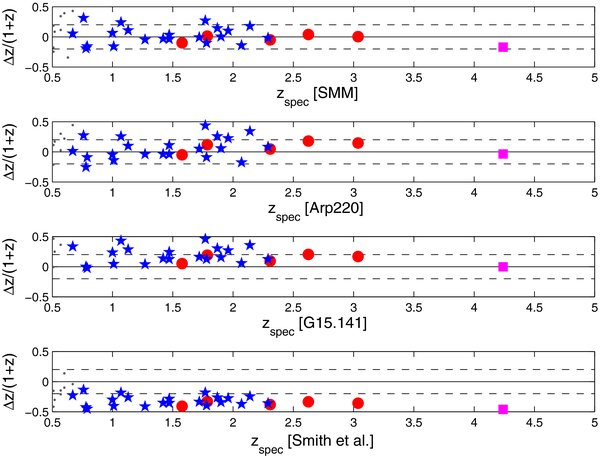
\includegraphics[width=14cm]{3_Redshift_Hatlas/apj404107f3_lr.jpg}
    \end{center}
    \vspace{-5mm}
    \caption{\small Comparación del \rt\ espectroscópico con el \rt\ fotométrico obtenido mediante el ajuste por mínimos tomando como referencia cuatro SEDs diferentes. Figura extraída del artículo \cite{article:Lapi_2011}.} 
    \label{fig:redshift_comparacion}
\end{figure}

Otra posible causa de error en la estimación del \rt\ proviene de la gran variedad de las galaxias con una tasas de formación estelar elevadas. Para estudiar cómo afecta la diversidad de galaxias en la estimación del \rt\ generaron una muestra de \maths{9\times{10}^{3}} galaxias a las que asignaron aleatoriamente un \rt\ comprendido entre \maths{1\geqslant\!z\!\geqslant 3.5} y una \sed\ procedente de un conjunto de 19 galaxias con una \sed\ bien conocida, todas ellas con una \sfr s \maths{\geqslant\,}\tfe{20} y una contribución del núcleo galáctico activo al flujo en el IR-Lejano inferior al \porcentaje{10} (a los \comillas{flujos simulados} de \microm{250}, \microm{350} y \microm{500} se les asignaron errores de forma aleatoria a partir de errores procedentes de observaciones reales). 
El siguiente paso fue calcular el \rt\ fotométrico de la muestra simulada utilizando como referencia la \sed\ de las galaxias \arp, \gquince\ y \smm. Después, corrigieron los valores del \rt\ fotométrico a partir de las desviaciones medias obtenidas en el estudio anterior y realizaron el histograma de la Figura \ref{fig:sed_distrib_simulacion}, reconociendo que la distribución de los \rts\ obtenidos solo se ve moderadamente afectada por la elección de la SED.

\begin{figure}[htb]
    \begin{center}
         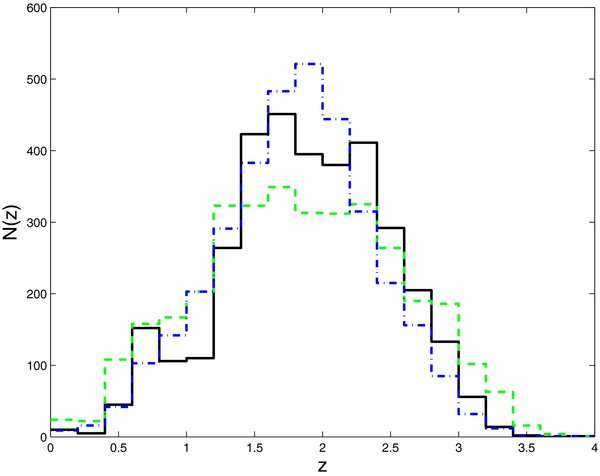
\includegraphics[width=14cm]{3_Redshift_Hatlas/simulacion_rt_distribution.jpg}
    \end{center}
    \vspace{-5mm}
    \caption{\small Distribución del \rt\ fotométrico, para las fuentes de la muestra con \maths{9\times{10}^{3}} galaxias simuladas, tomando como referencia la SED \smm\ (curva negra continua), tomando como referencia la SED de la galaxia Arp 220 (curva discontinua verde) y la SED de la galaxia G15.141 (curva discontinua azul). La figura pertenece al artículo \cite{article:Lapi_2011}.}
    \label{fig:sed_distrib_simulacion}
\end{figure}

A partir de estos estudios concluyeron que, si bien los \rt\ obtenidos son muy parecidos independientemente del modelo que tomemos como referencia (cualquiera de los considerados), la SED de la galaxia \smm\ resulta la más adecuada para realizar los ajustes. 

\newpage
\subsubsection{La galaxia \smm.}
La galaxia \smm\ ha sido cuidadosamente estudiada y se dispone de información detallada sobre ella. Como nos explican en \cite{article:smmj} se trata de una galaxia que muestra un \rt\ \maths{z=2.3259\pm0.0001} y que ha sido gravitatoriamente magnificada un factor \maths{\mu=32.5\pm4.5} por un grupo de galaxias con z=0.325. Es una galaxia especialmente brillante en el infrarrojo, con un flujo \flujo{870}=\mjy{\:106.0\,\pm\,7.0}. Su tasa de formación estelar es \sfr~=~\tfe{210\;\pm\;50} y se estima que la cantidad de materia bariónica es de \masassolares{M_{bar}=(4\pm2)\times{10}^{10}} siendo \maths{\sim 75\%} masa estelar y el resto gas y polvo. 

En la Figura \ref{fig:sed_lambda} se muestra la representación de la radiancia espectral (normalizada a \maths{5570}~\AA) \maths{S_{\lambda}} de la galaxia a partir de la interpolación lineal de los puntos del fichero que utilizamos como referencia. 
El máximo de emisión en el IR-lejano puede observase sobre los \maths{10^{6}}~\AA~\maths{\equiv 100\:\mu \mathrm{m}} (el máximo se aprecia mejor en la representación \maths{S_{\nu}}, Figura \ref{fig:sed_nu}).
Esta no es un curva obtenida de forma completamente experimental; se parte de un conjunto de puntos reducido (del orden de una decena) y después a partir de modelos teóricos\footnote{En \cite{article:Nuevo_2012} y \cite{article:Lapi_2011} se indica que las SEDs que ellos utilizan han sido modeladas utilizando el código GRASIL.}, se obtienen el resto de puntos de la curva que vemos. La zona \maths{\lambda \sim 50-500\;\mu \mathrm{m}} se modela a partir de las ecuaciones del cuerpo gris.
En realidad, el hecho de que los valores de los \rts\ obtenidos solo se vean moderadamente afectados por la elección de la SED, se debe en gran medida a que la información de la que se dispone de todas las galaxias consideradas como posible referencia en la Sección \ref{sec:selecion_sed} es limitada en esa zona del espectro\linebreak y cuando se modela la SED de cada una de ellas el resultado es parecido en todos los casos.

\begin{figure}[htb]
    \begin{center}
         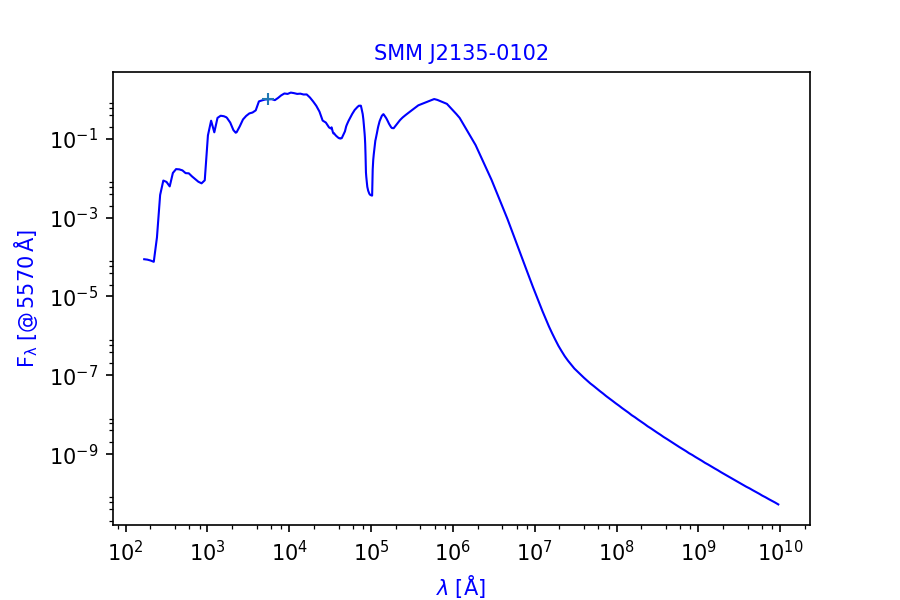
\includegraphics[width=14cm]{3_Redshift_Hatlas/grafica_SMM_F_lambda.png}
    \end{center}
    \vspace{-5mm}
    \caption{\small Representación en escala logarítmica del flujo \maths{F_{\lambda}} de la galaxia \smm\ normalizado a \angstrom{5570}. El punto en el que se encuentra el símbolo \maths{+} indica el punto de normalización.}
    \label{fig:sed_lambda}
\end{figure}

% Como se obtiene la sed se puede ver en Lapi et al(2011) pag 5
\newpage
\subsection{Algoritmo}

El \rt\ se obtiene mediante un ajuste de mínimos \maths{{\chi}^{2}} de la \sed\ normalizada de la galaxia \smm\ a los tres puntos experimentales proporcionados por el instrumento \spire. 
La \sed\ de la galaxia modelo se obtiene a partir de un fichero con dos columnas; la primera contiene los valores de la longitud de onda en \AA, la segunda los valores la densidad espectral de flujo\footnote{La SWIRE \anglicismo{Template Library} contiene la SED de 25 galaxias que se pueden utilizar como modelo: \url{http://www.iasf-milano.inaf.it/~polletta/templates/swire_templates.html}. La SED de la galaxia \smm\ ("The Cosmic Eyelash") que se utiliza en este trabajo, no se encuentra en esa librería, pero sigue la misma normalización.} \maths{F_{\lambda}}, normalizado a \angstrom{5570}. El flujo expresado en unidades de \maths{F_{\lambda}} tiene dimensiones de \maths{\mathrm{[M\,{L}^{-1}\,{T}^{-3} ]}}, sin embargo las medidas del \spire\ se encuentran en \jy{}, que es una unidad de \maths{F_{\nu}} con dimensiones de \maths{\mathrm{[M \,{T}^{-2} }]}. Para pasar de una unidad a la otra es suficiente tener en cuenta la relación \maths{|F_{\lambda}\mathrm{d}\lambda|=|F_{\nu}\mathrm{d}\nu|} . Los valores del flujo espectral que no se encuentran en el fichero se obtienen mediante interpolación lineal.

Para realizar el ajuste se tomarán dos parámetros, que denominaremos \paramc\ y \paramk. La curva de ajuste se obtiene multiplicando los valores del flujo por \paramc\ y los valores de la longitud de onda por \paramk.
En el sentido matemático, el ajuste consiste en una dilatación (o contracción) de la \sed\ de referencia en la dirección de cada uno de los ejes de coordenadas.

En el sentido físico la dilatación el en el eje \maths{y} podría interpretarse como un factor que indica cómo de luminosa es la galaxia considerada respecto de la galaxia de referencia. Sin embargo, la curva de referencia que se ha utilizado, está normalizada para un valor concreto de \maths{\lambda} por lo que no conocemos cuáles son las unidades físicas. Nos serviría para comparar magnitudes relativas entre los objetos del catálogo.
La dilatación en \maths{\lambda} se corresponde con un desplazamiento al rojo del espectro electromagnético con respecto a la \sed\ de referencia. Para entender cómo se relaciona el parámetro de ajuste \paramk\ con el \rt, \z, podemos verlo del siguiente modo:  Dado que la \sed\ de referencia no tiene \rt\ puesto que se supone que es la \sed\ de la galaxia \smm\ en un sistema en reposo (también habiendo corrigiendo el \rt\ debido al corrimiento al rojo cosmológico), esta curva nos daría la longitud de onda de emisión, \maths{{\lambda}_{e}}. La longitud de onda que observada\footnote{El nombre desplazamiento al rojo sugiere inmediatamente la posibilidad de realizar un ajuste mediante un \comillas{desplazamiento} de la \sed\ de referencia sobre el eje \maths{x}, sin embargo esto carece de sentido físico. Si en vez de multiplicar por \paramk\ consideramos una traslación del tipo \maths{{\lambda}_{o}={\lambda}_{e} + K} y sustituimos en la Ecuación \ref{eq:z_general} obtendremos

\begin{equation*}
 z = \frac{{\lambda}_{o} - {\lambda}_{e}}{{\lambda}_{e}} = \frac{{\lambda}_{o} - ({\lambda}_{o} + K) }{ {\lambda}_{o} + K } .
\end{equation*}

Esto no puede ser, porque obtendríamos un \rt\ diferente dependiendo de qué valor de \maths{\lambda} estuviésemos midiendo. 

} se corresponderá con la obtenida a partir del ajuste, es decir, \maths{{\lambda}_{o}={\lambda}_{e} \times K}, por tanto, utilizando la definición general de corrimiento al rojo,

\begin{equation*}
 z = \frac{{\lambda}_{o} - {\lambda}_{e}}{{\lambda}_{e}} = \frac{{\lambda}_{o} - \frac{{\lambda}_{o}}{K} }{ \frac{{\lambda}_{o}}{K} } = \frac{ ({\lambda}_{o} \times K) - {\lambda}_{o}}{{\lambda}_{o}} = K - 1.
\end{equation*}

La función del programa escrito en \python\ hace uso de esta relación para calcular \z.

\begin{figure}[htb]
    \begin{center}
         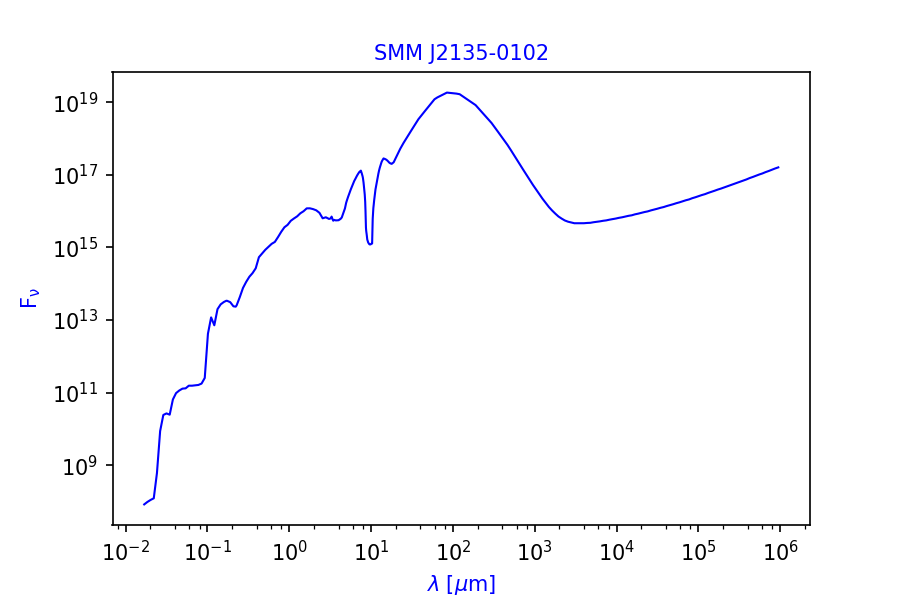
\includegraphics[width=14cm]{3_Redshift_Hatlas/grafica_SMM_F_nu.png}
    \end{center}
    \vspace{-5mm}
    \caption{\small \sed\ de la galaxia \smm. A diferencia de la Figura~\ref{fig:sed_lambda}, en este caso se está representando \maths{F_{\nu}} en vez de \maths{F_{\lambda}}. Esta curva es la que se utilizará como referencia para los ajustes. La zona \maths{\lambda \sim 50-500\;\mu \mathrm{m}} ha sido modelada como suma de dos cuerpos grises con temperaturas \maths{{T}_{d}\approx30\;\mathrm{K}} y \maths{{T}_{d}\approx60\;\mathrm{K}} y unos índices de emisividad para el polvo de \maths{\beta=1.7} y \maths{\beta=2} respectivamente.}
    \label{fig:sed_nu}
\end{figure}

\begin{figure}[H]
  \begin{center} 
  
    \subfloat[]{
     \label{subfig:ajuste_a}
      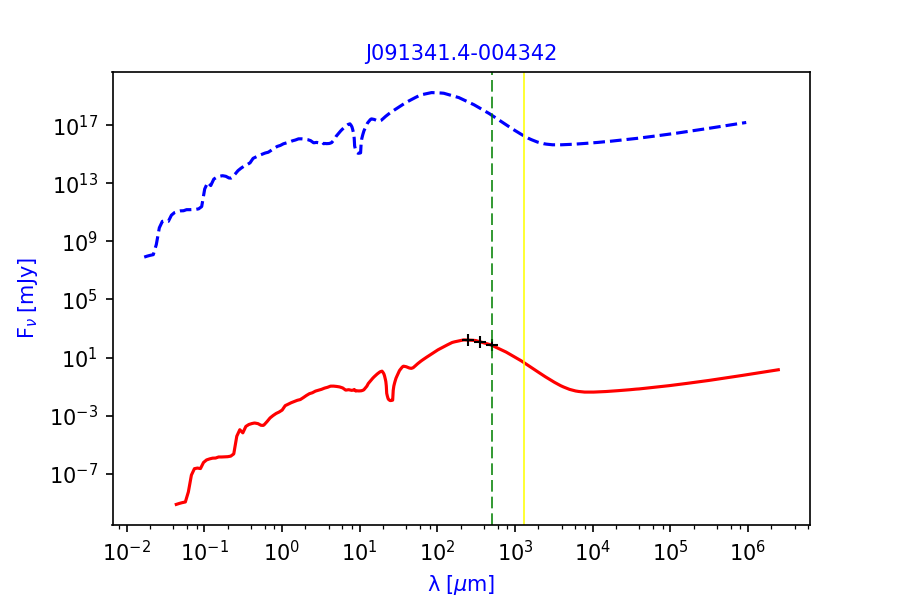
\includegraphics[width=0.8\textwidth]{3_Redshift_Hatlas/ajuste_6.png}} 
      
    \subfloat[]{
     \label{subfig:ajuste_b}
      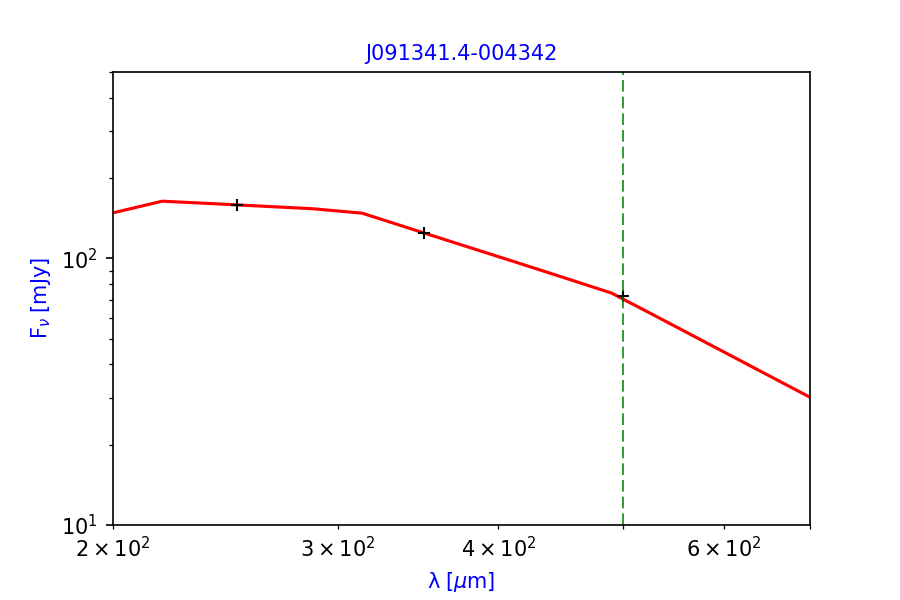
\includegraphics[width=0.8\textwidth]{3_Redshift_Hatlas/ajuste_6_zoom.png}}

  \end{center}
    
  \caption{\small Ajuste por mínimos cuadrados de la SED de la galaxia \smm\ para el objeto J091341.4-004342 del catálogo \hatlas. En la figura \ref{subfig:ajuste_a}, la curva discontinua es la curva mostrada en la Figura \ref{fig:sed_nu}. La curva continua es la curva del ajuste, que se encuentra sobre los tres puntos experimentales de un objeto, que vienen representados por el símbolo '+'. Al utilizar la representación logarítmica, en cada uno de los ejes, la curva roja aparenta ser un desplazamiento de la curva azul. Las líneas verticales se utilizan para visualizar el desplazamiento horizontal relacionado con el desplazamiento al rojo \z. En el caso del eje~\maths{x} el desplazamiento será \maths{\log_{10}{(z+1)}}. En la figura \ref{subfig:ajuste_b} se muestra con más detalle la zona de encuentro de la curva de ajuste con los puntos experimentales. Se aprecia perfectamente que la curva roja se compone de segmentos unidos, debido a que solo conocemos un conjunto de \maths{\sim1000} valores de la \sed\, el resto se obtiene mediante interpolación lineal a partir de estos.}
\end{figure}

\subsection{Confrontación del método}

Cabe señalar que en este trabajo no se ha probado que el método descrito en esta sección proporcione ajustes válidos para obtener el \rt\ fotométrico de las ETGs. Para hacer eso, deberíamos disponer de una muestra suficientemente grande de fuentes con \rt\ espectroscópico para poder comparar los valores obtenidos con una referencia fiable. Aunque no disponemos de esa información, en el artículo~\cite{article:Nuevo_2012} se ha publicado una tabla con el valor del \rt\ de 64 galaxias que ellos calcularon utilizando su propio programa. En la Figura~\ref{fig:redshift_comparacion} se ha hecho un ajuste para comparar sus resultados con los nuestros.  

\vspace*{-15mm}

\begin{figure}[h]
    \begin{center}
         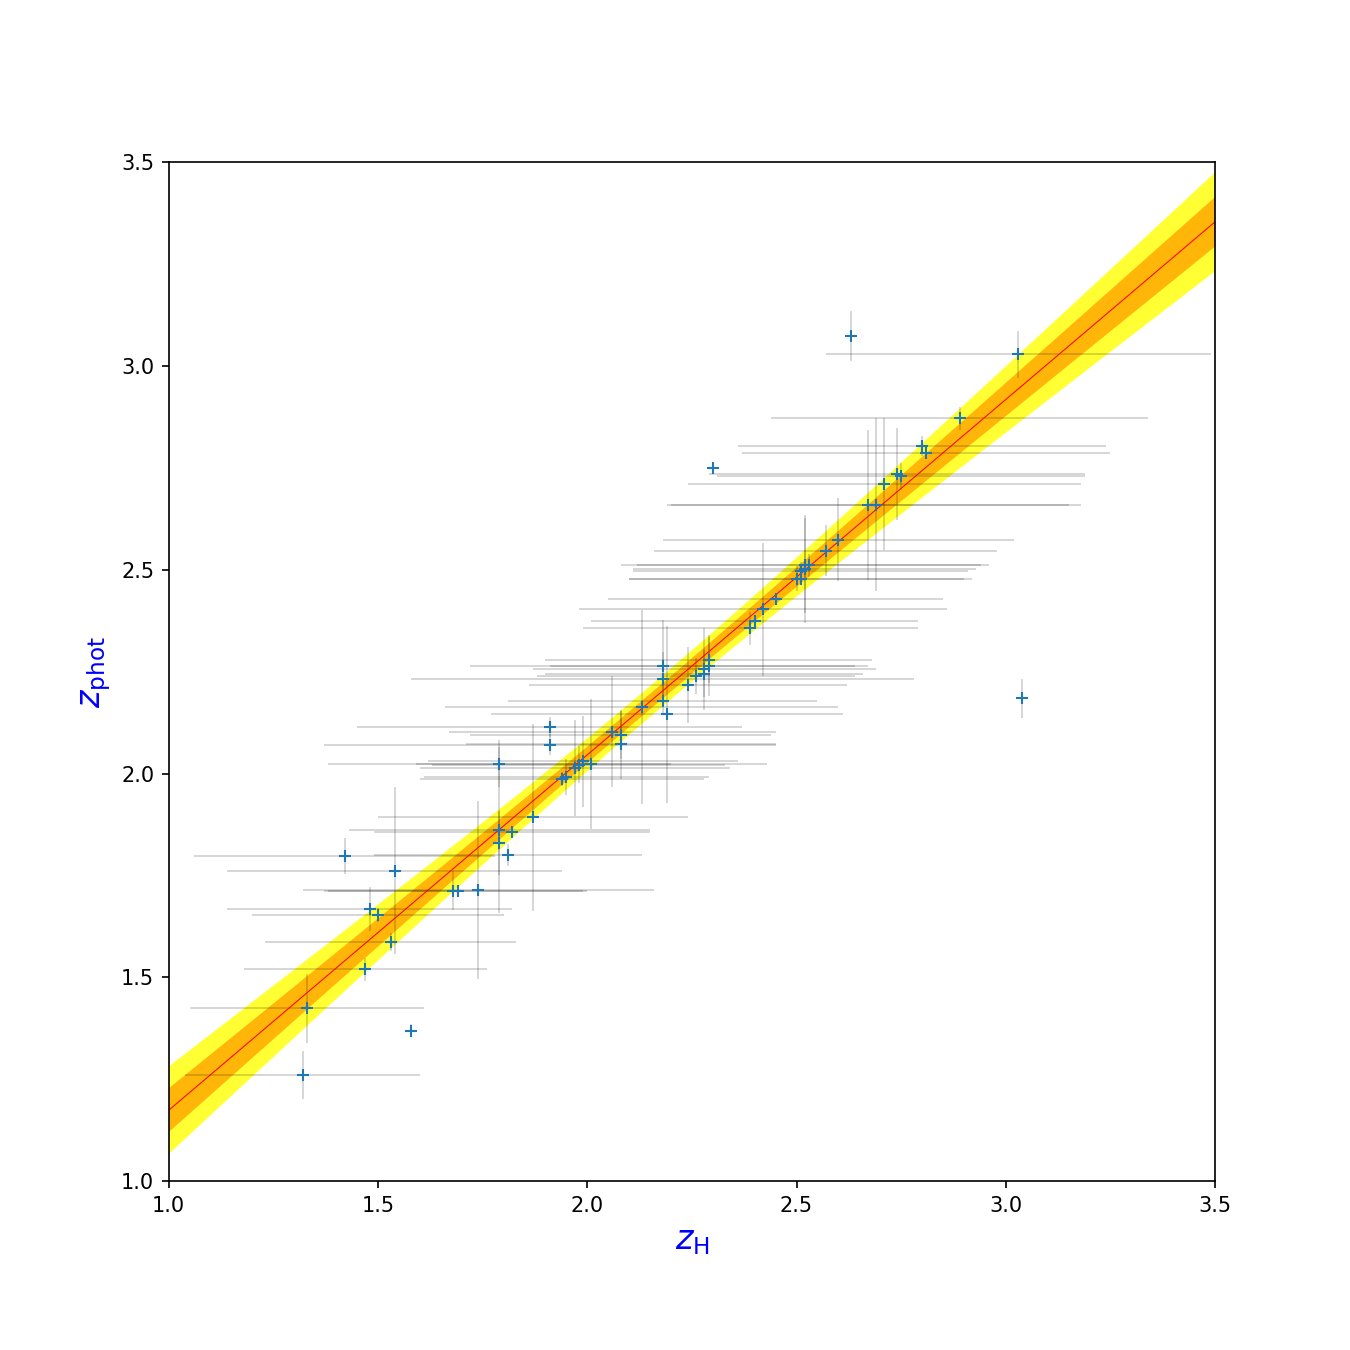
\includegraphics[width=16cm]{3_Redshift_Hatlas/comparacion_Z.png}
    \end{center}
    \vspace*{-15mm}
    \caption{\small Comparación del \rt\ fotométrico obtenido utilizando el algoritmo descrito en la Sección~\ref{sec:3_redshift_hatlas}, \maths{z_{\mathrm{phot}}}, con los valores del \rt\ fotométrico estimado por \cite{article:Nuevo_2012}, \maths{z_{\mathrm{H}}}. La linea roja representa el ajuste lineal, \maths{{z}_{\mathrm{phot}}=(0.87 \pm 0.04)\times {z}_{\mathrm{H}}+(0.3 \pm 0.1)}. La zona anaranjada representa la zona con una confianza \maths{\sigma<1} y la amarillenta \maths{\sigma<2}. Las barras de error no se han tenido en cuenta para realizar el ajuste. Las barras de error horizontales se corresponden los los valores asignados a las medidas que aparecen en el artículo, las barras de error verticales se obtienen a partir de la varianza del ajuste proporcionado por el programa que aparece en la Sección \ref{apendice:codigo:rojo} (Los valores utilizados para realizar la gráfica se encuentran en la Tabla~\ref{tab:redshift_halos}).} 
    \label{fig:comparacion_sed}
\end{figure}

La tabla del artículo no solo proporciona los valores del \rt\ fotométrico que ellos obtuvieron, también los valores de la desviación estándar que ellos asignaron a estas medidas. Al no disponer de una muestra de referencia con la que realizar estudios estadísticos, tampoco disponemos de los recursos suficientes para asignar valores a \maths{\sigma^z}. Para asignar los valores de \maths{{\sigma}^z} a los \linebreak
\\
valores \maths{z_{\mathrm{phot}}} obtenidos mediante nuestro método, se ha realizado un ajuste similar al mostrado en la Figura~\ref{fig:ajuste_error_gama}, partiendo de las desviaciones estándar asignadas a los desplazamientos al rojo del ajuste realizado en el artículo (Figura~\ref{fig:ajuste_errores_ajuste}).

\vspace*{-1mm}

\begin{figure}[h]
    \begin{center}
         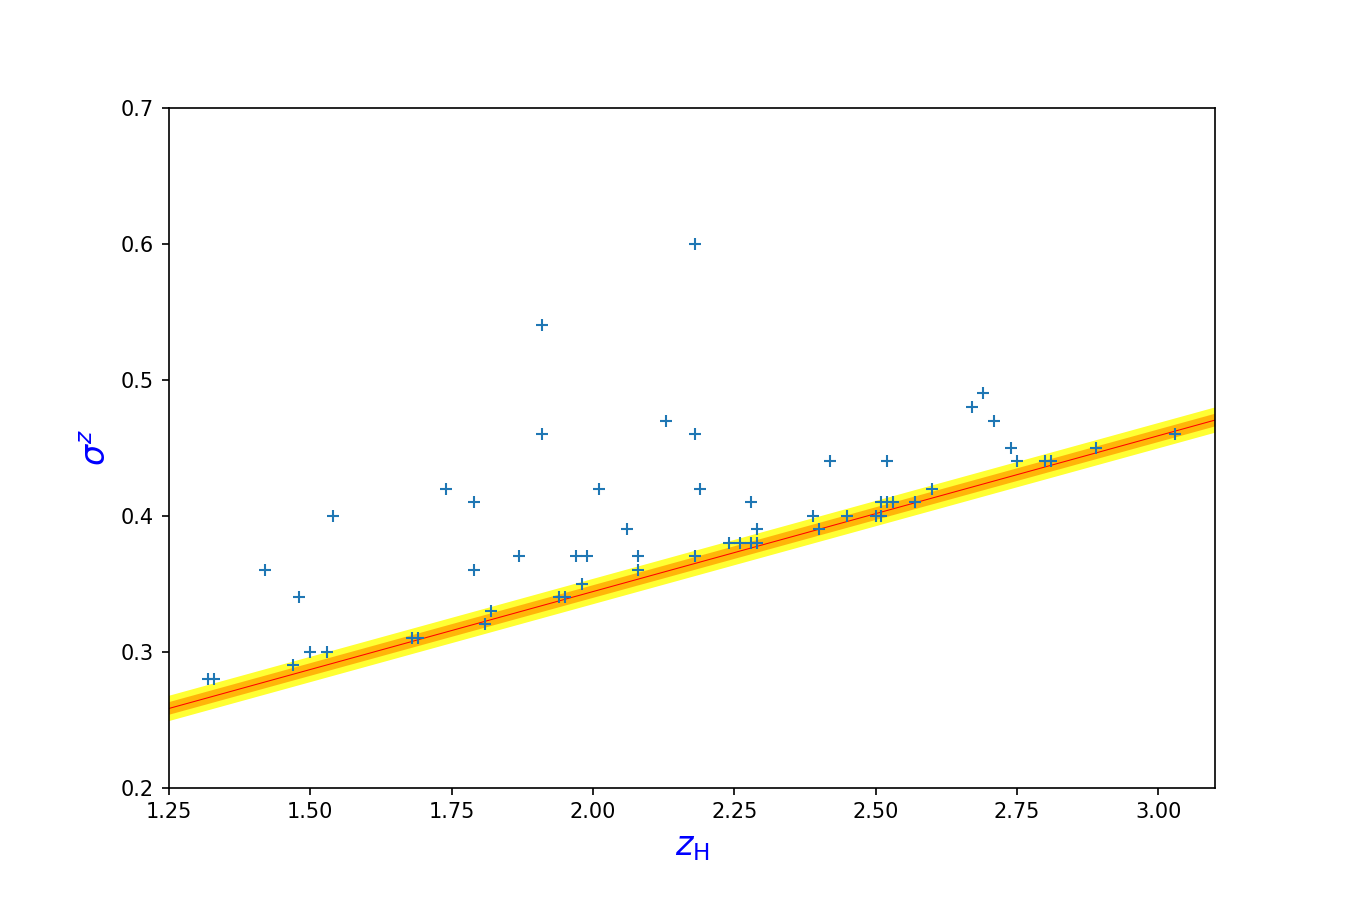
\includegraphics[width=16cm]{3_Redshift_Hatlas/ajuste_errores.png}
    \end{center}
    \vspace*{-10mm}
    \caption{\small Representación de la desviación estándar del \rt, \maths{{\sigma}^{z}} en función de \maths{z_{\mathrm{H}}}. Los valores de los puntos representados se encuentran en la Tabla~\ref{tab:redshift_halos}. La recta se ha obtenido mediante un ajuste lineal de la forma \maths{{\sigma}^z= a\times(1+z)} con \maths{a} como parámetro de libre. El parámetro resultante del ajuste ha sido \maths{a=0.115\pm 0.005}.}
    \label{fig:ajuste_errores_ajuste}
\end{figure}


\vspace*{-1mm}


